\input{preambulo_presentacion_Berlin_beaver}
\usepackage{pifont}
\usepackage{siunitx}
\usetikzlibrary{shapes}
\newcommand{\cmark}{\ding{51}}%
\newcommand{\xmark}{\ding{55}}%
\definecolor{cadmiumgreen}{rgb}{0.0, 0.42, 0.24}
\makeatletter
\setbeamertemplate{footline}
{
  \leavevmode%
  \hbox{%
  \begin{beamercolorbox}[wd=.333333\paperwidth,ht=2.25ex,dp=1ex,center]{section in foot}%
    \usebeamerfont{section in foot} \insertsection
  \end{beamercolorbox}%
  \begin{beamercolorbox}[wd=.333333\paperwidth,ht=2.25ex,dp=1ex,center]{subsection in foot}%
    \usebeamerfont{subsection in foot}  \insertsubsection
  \end{beamercolorbox}%
  \begin{beamercolorbox}[wd=.333333\paperwidth,ht=2.25ex,dp=1ex,right]{date in head/foot}%
    \usebeamerfont{date in head/foot} \insertshortdate{} \hspace*{2em}
    \insertframenumber{} / \inserttotalframenumber \hspace*{2ex} 
  \end{beamercolorbox}}%
  \vskip0pt%
}
\makeatother
%--------------------------------------------------------------------
%--------------------------------------------------------------------
\newcounter{choice}
\renewcommand\thechoice{\Alph{choice})}
%\newcommand\choicelabel{\thechoice.}
\newcommand\choicelabel{\thechoice}

\newenvironment{choices}%
  {\list{\choicelabel}%
     {\usecounter{choice}\def\makelabel##1{\hss\llap{##1}}%
       \settowidth{\leftmargin}{W.\hskip\labelsep\hskip 2.5em}%
       \def\choice{%
         \item
       } % choice
       \labelwidth\leftmargin\advance\labelwidth-\labelsep
       \topsep=0pt
       \partopsep=0pt
     }%
  }%
  {\endlist}

\newenvironment{oneparchoices}%
  {%
    \setcounter{choice}{0}%
    \def\choice{%
      \refstepcounter{choice}%
      \ifnum\value{choice}>1\relax
        \penalty -50\hskip 1em plus 1em\relax
      \fi
      \choicelabel
      \nobreak\enskip
    }% choice
    % If we're continuing the paragraph containing the question,
    % then leave a bit of space before the first choice:
    \ifvmode\else\enskip\fi
    \ignorespaces
  }%
  {}
%----------------------------------------------------------
%----------------------------------------------------------

\setbeamertemplate{navigation symbols}{}
\date{22 de marzo de 2021}
\title{Sesión 6. Matemáticas}
\subtitle{Asesoría}
\begin{document}
\maketitle
\fontsize{14}{14}\selectfont
\spanishdecimal{.}
\section*{Contenido}
\frame[allowframebreaks]{\tableofcontents[currentsection, hideallsubsections]}
\section{Resultados fracciones}
\frame{\tableofcontents[currentsection, hideothersubsections]}

\subsection{Resultado de las fracciones}

\begin{frame}
\frametitle{Resultado de las restas}
\setbeamercolor{item projected}{bg=blue!70!black,fg=yellow}
\setbeamertemplate{enumerate items}[circle]
\begin{enumerate}[<+->]
\item $R=1/3$
\item $R=1/2$
\item $R=1/3$
\item $R=1/12$
\end{enumerate}
\end{frame}
\begin{frame}
\frametitle{Resultado de las operaciones mixtas}
\setbeamercolor{item projected}{bg=blue!70!black,fg=yellow}
\setbeamertemplate{enumerate items}[circle]
\begin{enumerate}[<+->]
\item $R=1 \, 5/12$
\item $R=17/24$
\item $R=35/36$
\item $R=4/5$
\end{enumerate}
\end{frame}

\section{Relación de igualdad}
\frame{\tableofcontents[currentsection, hideothersubsections]}
\subsection{Definición}

\begin{frame}
\frametitle{La relación de igualdad}
En matemáticas el concepto de igualdad es muy importante, ya que establece una relación entre dos cantidades.
\\
\bigskip
\pause
La igualdad es una regla que debe de mantenerse en todo momento, ya que podemos ocupar alguna de esas cantidades, pero hay que \emph{equilibrar} la otra cantidad, para mantener la igualdad.
\end{frame}
\begin{frame}
\frametitle{Ejemplo}
Veamos el siguiente caso:
\pause
\begin{align*}
a = a
\end{align*}
\pause
Donde $a$ puede ser cualquier valor, en este caso, se le conoce como \emph{variable}. \pause Este es un resultado que parece muy directo, y de hecho lo es, pero lo vamos a ocupar para discutir la importancia de mantener una igualdad.
\end{frame}
\begin{frame}
\frametitle{Ejemplo con variantes}
Si de la relación de igualdad:
\begin{align*}
  a = a
\end{align*}
\pause
Le sumamos una cantidad a un elemento, digamos el del lado izquierdo:
\begin{align*}
a + b \neq a
\end{align*}
\pause
el signo $\neq$ nos dice que los elementos del lado izquierdo y derecho, \textbf{no son iguales}. 
\end{frame}
\begin{frame}
\frametitle{Ejemplo con variantes}
Para mantener la igualdad, debemos de sumar la misma cantidad del lado derecho, con esto, la igualdad se mantiene:
\pause
\begin{align*}
a + b = a + b
\end{align*}
\end{frame}
\begin{frame}
\frametitle{Ejemplo con variantes}
Para cada operación aritmética que se aplique a un lado de la igualdad, se debe de realizar la misma operación al lado contrario de la igualdad:
\begin{eqnarray*}
a - c &\neq& a \\ \pause
a - c &=& a - c \\ \pause
a &\neq& a * d \\ \pause
a * d &=& a * d \\ \pause
\end{eqnarray*}
\end{frame}
\begin{frame}
\frametitle{Ejemplo con variantes}
Para cada operación aritmética que se aplique a un lado de la igualdad, se debe de realizar la misma operación al lado contrario de la igualdad:
\begin{eqnarray*}
\dfrac{a}{m} &\neq& a \\ \pause
\dfrac{a}{m} &=& \dfrac{a}{m}
\end{eqnarray*}
\pause
Hay que tomar en cuenta que ahora, todas las operaciones aritméticas están consideradas, es decir, debemos de contemplar tanto la potenciación como la radicación de una variable.
\end{frame}
\begin{frame}
\frametitle{Potenciación}
Cuando se ocupa la potencia de una variable en una expresión, debemos de elevar a la misma potencia, el lado contrario:
\pause
\begin{eqnarray*}
a &=& a \\ \pause
(a)^{2} &\neq& a \\ \pause
(a)^{2} &=& (a)^{2}
\end{eqnarray*}
\end{frame}
\begin{frame}
\frametitle{Radicación}
Es muy común la raíz cuadrada, pero también se ocupan las raíces cúbica, cuarta, etc.
\pause
\begin{eqnarray*}
b &=& b \\ \pause
\sqrt{b} &\neq& b \\ \pause
\sqrt{b} &=& \sqrt{b} \\ \pause
\sqrt[3]{d} &\neq& d \\ \pause
\sqrt[3]{d} &=& \sqrt[3]{d} \\ \pause
\end{eqnarray*}
\end{frame}
\begin{frame}
\frametitle{Expresiones más elaboradas}
En matemáticas tendremos desarrollos en donde las expresiones involucran más elementos, y debemos de recordar siempre en una igualdad, ambos lados tienen que estar equilibrados:
\pause
\begin{eqnarray*}
a + b + c &=& a + b + c \\ \pause
a + b + c + d &\neq& a + b + c \\ \pause
a + b + c + d &=& a + b + c + d \\ \pause
\end{eqnarray*}
\end{frame}
\begin{frame}
\frametitle{Cuidado con dos operaciones}
Cuando las expresiones son más elaboradas, hay que tener cuidado con la potenciación y radicación por que cuando se involucran más elementos, la manera de equilibrar la expresión es distinta.
\end{frame}
\begin{frame}
\frametitle{Casos especiales}
Ejemplos:
\begin{eqnarray*}
a + b &=& a + b \\ \pause
(a + b)^{2} &\neq& (a + b) \\ \pause
(a + b)^{2} &\neq& a^{2} + b^{2}
\end{eqnarray*}
\end{frame}

\section{Repaso de álgebra}
\frame{\tableofcontents[currentsection, hideothersubsections]}
\subsection{Conceptos}

\begin{frame}
\frametitle{Expresión algebraica}
Es la representación de un símbolo algebraico (literal) o de alguna o más operaciones algebraicas.
\pause
Ejemplos:
\begin{align*}
a, \hspace{0.5cm} 5 \, x, \hspace{0.5cm} \sqrt{4 \, a}, \hspace{0.5cm} (a + b) \, c, \hspace{0.5cm} \dfrac{(5 \, x - 3 \, y) a}{x^{2}}
\end{align*}
\end{frame}
\begin{frame}
\frametitle{Término}
Es una expresión algebraica que cosnta de un solo símbolo o de varios símbolos \emph{no separados} entre sí por el signo $+$, $-$ o $*$.
\pause
Ejemplos de términos
\begin{align*}
a, \hspace{0.5cm} 3 \, b, \hspace{0.5cm} -2 \, x \, y, \hspace{0.5cm} \dfrac{4 \, a}{3 \, x}
\end{align*}
\end{frame}
\begin{frame}
\frametitle{Elementos de un término}
Los elementos de un término son \textcolor{blue}{cuatro}:
\\[2em]
\pause
\begin{figure}[H]
\begin{tikzpicture}[overlay]
  \node at (1, 1) {$-3 \, x^{2}$}; \pause
  \draw [thick, ->] (0, 0) -- (0.5, 0.7);
  \node at (-0.3, -0.3) {Signo}; \pause
  \draw [thick, ->] (1, -1) -- (1, 0.7);
  \node at (0.5, -1.2) {Coeficiente}; \pause
  \draw [thick, ->] (2, -0.5) -- (1.3, -0.5) -- (1.3, 0.7);
  \node at (2.8, -0.5) {Literal}; \pause
  \draw [thick, ->] (2.5, 1.1) -- (1.7, 1.1);
  \node at (3.7, 1.1) {Exponente};

\end{tikzpicture}
\end{figure}
\end{frame}
\begin{frame}
\frametitle{¿Cuáles son los elementos de los siguientes términos?}
\begin{align*}
-x, \hspace{1cm} - 5 \, b \, c \hspace{1cm} \dfrac{3 \, a}{2 \, b}
\end{align*}
\end{frame}
\begin{frame}
\frametitle{El grado de un término}
El grado de un término es el valor mayor del exponente de las literales que contenga el término.
\pause
\begin{align*}
b \, x^{3} \hspace{1cm} 4 \, x^{2} \, y^{4}
\end{align*}
\pause
Toma en cuenta de que si aparecen más literales, se debe de indicar el grado del término para cada literal.
\end{frame}
\begin{frame}
\frametitle{El grado de un término}
En el ejemplo:
\begin{align*}
4 \, x^{2} \, y^{4}
\end{align*}
\pause
Se tiene que:
\setbeamercolor{item projected}{bg=blue!70!black,fg=yellow}
\setbeamertemplate{enumerate items}[circle]
\begin{enumerate}[<+->]
\item Con respecto a $x$, el término es de segundo grado.
\item Con respecto a $y$, el término es de cuarto grado.
\end{enumerate}
\end{frame}

\subsection{Clasificación de las expresiones}

\begin{frame}
\frametitle{El monomio}
Un monomio es una expresión algebraica que consta de un solo término:
\begin{align*}
3 \, a \hspace{1cm} - 5 \, b \hspace{1cm} \dfrac{x^{2} \, y}{4 \, a^{3}}
\end{align*}
\end{frame}
\begin{frame}
\frametitle{El binomio}
Un binomio es una expresión que consta de dos términos:
\begin{align*}
a + b \hspace{1cm} x - y \hspace{1cm} \dfrac{a^{2}}{3} - \dfrac{5 \, m \, x^{4}}{6 \, b^{2}}
\end{align*}
\end{frame}
\begin{frame}
\frametitle{El trinomio}
Es una expresión que consta de tres términos:
\begin{align*}
a + b + c \hspace{1cm} x^{2} - 5 \, x + 6 \hspace{1cm} 5  \, x^{2} - 6 \, y^{3} + \dfrac{a^{2}}{3}
\end{align*}  
\end{frame}
\begin{frame}
\frametitle{Un polinomio}
Es una expresión algebraica que consta de más de un término:
\begin{align*}
a + b \hspace{1cm} a + x - y \hspace{1cm} x^{3} + 2 \, x^{2} +  x +  7
\end{align*}
\pause
Notarás que tanto un binomio como un trinomio, éstos son polinomios, pero es común llamar a esas expresiones de tal manera.
\end{frame}

\subsection{Clases de polinomios}

\begin{frame}
\frametitle{Polinomio entero}
Un polinomio es \emph{entero}: cuando ninguno de sus términos tiene un denominador:
\pause
\begin{align*}
x^{2} + 5 \, x - 6
\end{align*}
\end{frame}
\begin{frame}
\frametitle{Polinomio fraccionario}
Un polinomio es \emph{fraccionario}: cuando alguno de sus términos tiene un denominador:
\pause
\begin{align*}
\dfrac{a^{2}}{c} + \dfrac{a}{c} - 8
\end{align*}
\end{frame}
\begin{frame}
\frametitle{Polinomio racional}
Un polinomio es \emph{racional}: cuando no contiene radicales:
\pause
\begin{align*}
x^{2} + 5 \, x - 6 \hspace{1cm} \dfrac{a^{2}}{c} + \dfrac{a}{c} - 8
\end{align*}
\pause
Se llama polinomio \emph{irracional} cuando alguno de los términos contiene un radical:
\pause
\begin{align*}
\sqrt{a} + b - c + \sqrt{a \, b \, c}
\end{align*}
\end{frame}
\begin{frame}
\frametitle{Término independiente}
El término independiente de una polinomio con relación a una literal, es el término que no contiene ninguna literal:
\pause
\begin{align*}
a^{3} - a^{2} + 3 \, a - 5
\end{align*}
\pause
El término independiente con relación a la literal $a$, es $5$, por que no tiene $a$.
\end{frame}

\subsection{Términos semejantes}

\begin{frame}
\frametitle{Términos semejantes}
Dos o más términos son \emph{semejantes} cuando tiene la misma parte literal, es decir, cuando tienen la misma literal afectadas de iguales exponentes.
\pause
\begin{align*}
2 \, a \hspace{1cm} a \\
- 2 \, b \hspace{1cm} 8 \, b \\
5 \, a^{3} \, b^{2} \hspace{1cm} -8 \, a^{3} \, b^{2}
\end{align*}
\end{frame}ç
\begin{frame}
\frametitle{Términos no semejantes}
Los términos:
\begin{align*}
4 \, a \, b \hspace{1cm} - 6 \, a^{2} \, b
\end{align*}
no son semejantes, \pause aunque tienen las mismas literales, éstas \textbf{no tienen los mismos exponentes}.
\end{frame}
\subsection*{Reducción términos semejantes}
\begin{frame}
\frametitle{Reducción de dos términos semejantes}
Reducir los términos semejantes es una operación que tiene por objeto, \textcolor{red}{convertir en un solo término} dos o más términos semejantes.
\end{frame}
\begin{frame}
\frametitle{Suma de dos términos con el mismo signo}
\textbf{Regla: } Se suman los coeficientes, poniendo delante de esta suma el mismo signo que tienen todos los términos y a continuación, se escribe la parte literal:
\pause
\begin{eqnarray*}
3 \, a + 2 \, a &=& \pause 5 \, a \\[0.5em] \pause
-5 \, b -7 \, b &=& \pause - 12 \, b \\[0.5em] \pause
-a^{2} - 9 \, a^{2} &=& \pause - 10 \, a^{2}
\end{eqnarray*}
\end{frame}
\begin{frame}
\frametitle{Dos términos con distinto signo}
\textbf{Regla: } Se restan los coeficientes, poniendo delante de esta diferencia el signo del mayor, a continuación se escribe la parte literal.
\pause
\begin{eqnarray*}
2 \, a - 3 \, a &=& \pause - a \\
18 \, x - 11 \, x &=& \pause 7 \, x \\[0.5em]
\dfrac{1}{2}  \, a - \dfrac{2}{3} \, a &=& \pause \dfrac{1}{6} \, a
\end{eqnarray*}
\end{frame}
\begin{frame}
\frametitle{Dos o más términos con distintos signos}
\textbf{Regla: }
\setbeamercolor{item projected}{bg=blue!70!black,fg=yellow}
\setbeamertemplate{enumerate items}[circle]
\begin{enumerate}[<+->]
\item Se reducen a un solo término todos los positivos.
\item Se reducen a um solo término todos los negativos.
\item A los resultados obtenidos, se aplica la regla anterior.
\end{enumerate}
\end{frame}
\begin{frame}
\frametitle{Dos o más términos con distintos signos}
Ejemplo: Reducir: $5 a - 8 a + a - 6 a + 21 a$
\pause
Reduciendo los positivos: $5 a + a + 21 a =  27 a$.
\\
\bigskip
\pause
Reduciendo los negativos: $-8 a - 6 a =  -14 a$.
\\
\bigskip
\pause
Nos quedamos con $27 a - 14 a =$ \pause $13 a$
\end{frame}
\end{document}